\documentclass{article}
\usepackage[T1]{fontenc}
\usepackage{lmodern}
\usepackage{graphicx}
\usepackage{amsmath,amssymb}
\usepackage[a4paper,margin=2cm]{geometry}
\usepackage[absolute,overlay]{textpos}
\setlength{\TPHorizModule}{1mm}
\setlength{\TPVertModule}{1mm}
\usepackage[indonesian]{babel}
\usepackage{hyperref}
\setlength{\emergencystretch}{2em}
% unit: Halaman 18

\begin{document}

% === Halaman 18 (llm) ===

\vspace{95.04mm}

\section*{Enciphering}

\begin{itemize}
    \item Setiap blok plainteks mengalami 16 kali putaran \textit{enciphering}
    \item Setiap putaran \textit{enciphering} merupakan jaringan Feistel:
    \[
    \begin{aligned}
    L_i &= R_{i-1} \\
    R_i &= L_{i-1} \oplus f(R_{i-1}, K_i)
    \end{aligned}
    \]
\end{itemize}

\vspace{40mm}

\textbf{Gambar 4. Satu putaran \textit{enciphering}}

% deskripsi: Diagram alur proses enciphering secara keseluruhan yang melibatkan IP, 16 kali putaran enciphering, IP-1, dan key expansion.
% bbox normalisasi: [0.7200, 0.0000, 0.9800, 0.3200]
\begin{textblock*}{54.60mm}(151.20mm,0.00mm)
\noindent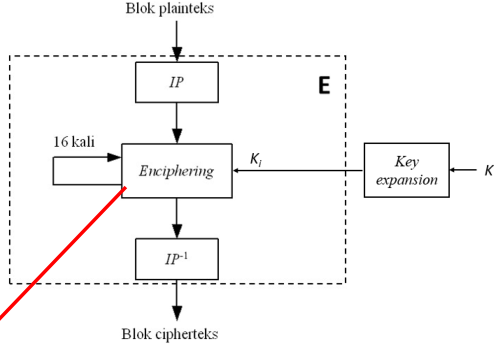
\includegraphics[width=54.60mm,height=95.04mm]{../../images/llm/page_018_img_01.png}%
\end{textblock*}

% deskripsi: Diagram detail satu putaran jaringan Feistel yang menunjukkan operasi XOR antara L_{i-1} dengan hasil fungsi f(R_{i-1}, K_i) untuk menghasilkan R_i, sementara R_{i-1} menjadi L_i.
% bbox normalisasi: [0.4000, 0.4400, 0.9300, 0.9000]
\begin{textblock*}{111.30mm}(84.00mm,130.68mm)
\noindent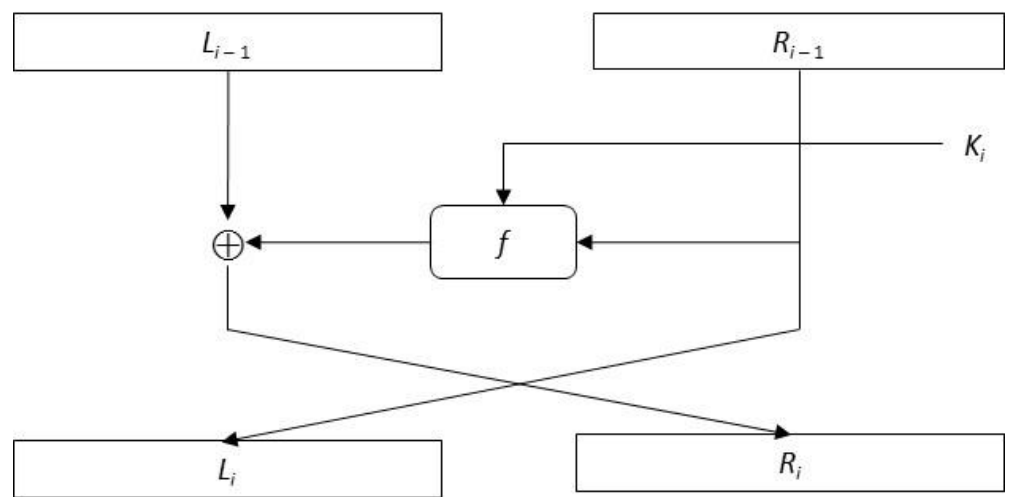
\includegraphics[width=111.30mm,height=136.62mm]{../../images/llm/page_018_img_02.png}%
\end{textblock*}

\end{document}
